
\documentclass{article}

\usepackage[latin1]{inputenc}
\usepackage{caption}

\usepackage{tikz}
\usetikzlibrary{arrows,calc,positioning,shadows,shapes,matrix}
\usetikzlibrary{fit,chains,arrows.meta,shapes.geometric}
\usetikzlibrary{datavisualization.formats.functions}

\usepackage[american,siunitx]{circuitikz}
\usepackage{pgfplots}
\usepackage{schemabloc,calc,blox}

\usepackage{pgfplots}
%\usepgfplotslibrary{external}
%\tikzexternalize[prefix=tikz/]

\usepackage[miktex]{gnuplottex}


\begin{document}
%\pagestyle{empty}

from https://tex.stackexchange.com/questions/9386/difference-between-right-of-and-right-of-in-pgf-tikz website.

centre-to-centre placing while using \texttt{right of=} option in tikz


\begin{tikzpicture}
\node (a) {loooooooooooooooooooooooooooooong};
\node[right of=a,font=\bfseries,blue] (b) {node b};
\end{tikzpicture}

boundary-to-boundary placing while using \texttt{right=of} option in tikz

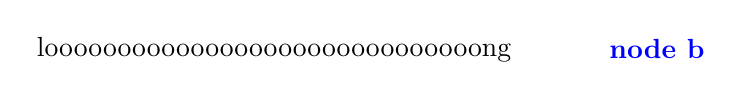
\begin{tikzpicture}
\node (a) {loooooooooooooooooooooooooooooong};
\node[right=of a,font=\bfseries,blue] (b) {node b};
\end{tikzpicture}




% ---------------------------------------------------------
\vspace{5ex}
Below demos are from https://tex.stackexchange.com/questions/209355/drawing-a-block-diagram-using-tikz website.

\begin{figure}[!htb]
%\centering
\resizebox{\textwidth}{!}{%
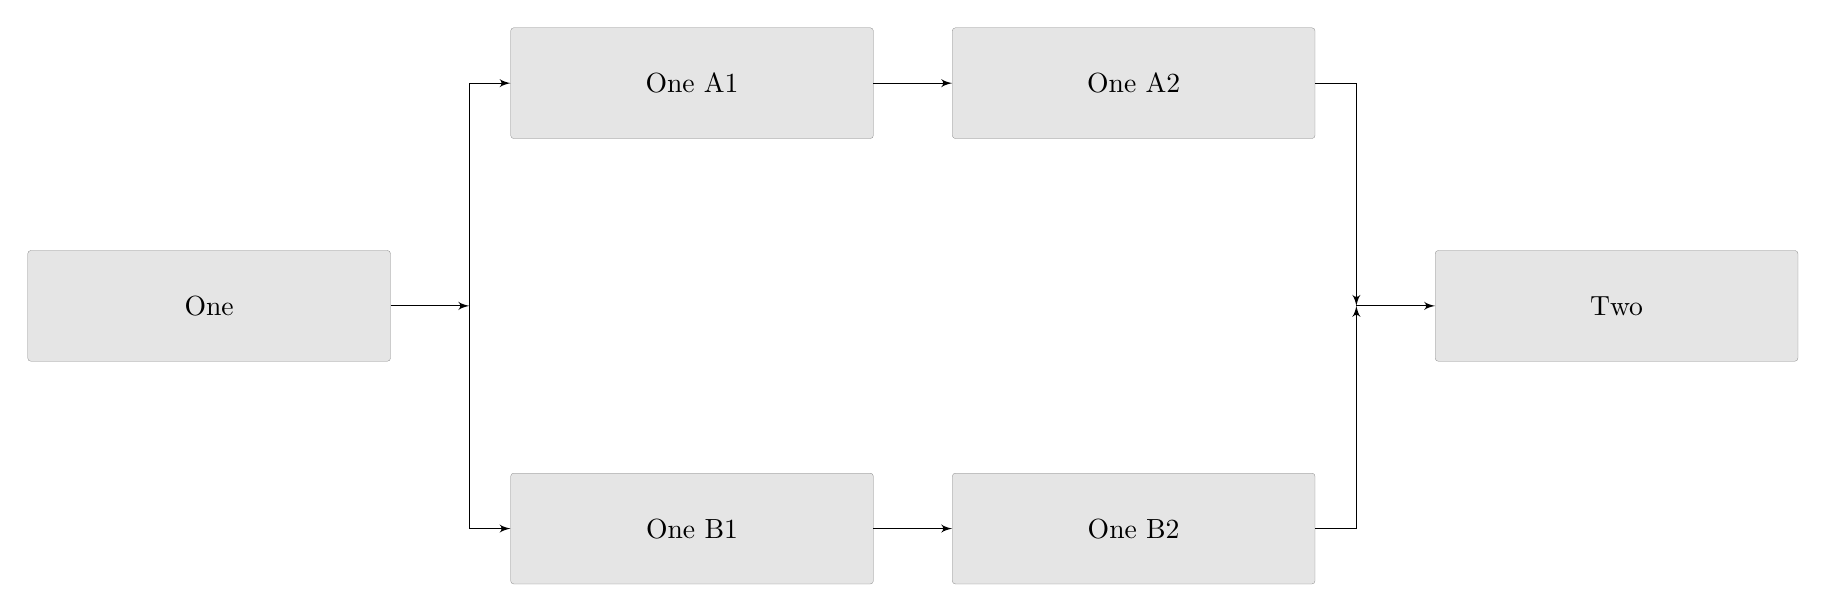
\begin{tikzpicture}[node distance=4cm,auto, > = latex']
\tikzstyle{line} = [draw, -latex']
\tikzset{label/.style={draw=gray, ultra thin, rounded corners=.25ex, fill=gray!20,text width=4cm, text badly centered,  inner sep=2ex, anchor=east, minimum height=4em}}
% Place nodes
\node [label] (one) {One};
\node [coordinate, right = 1cm of one] (onetemp){};
\node [label, above right of = onetemp] (onea1) {One A1};
\node [label, right = 1cm of onea1] (onea2) {One A2};
\node [label, below right of = onetemp] (oneb1) {One B1};
\node [label, right = 1cm of oneb1] (oneb2) {One B2};
\node [coordinate, below right of = onea2] (twotemp) {};
\node [label, right = 1cm of twotemp] (two){Two};

% Draw edges
\path [line] (one)-- (onetemp); 
\path [line] (onetemp) |- (onea1); 
\path [line] (onea1) -- (onea2);
\path [line] (onetemp) |- (oneb1);
\path [line] (oneb1) -- (oneb2);
\path [line] (oneb2) -| (twotemp);
\path [line] (onea2) -| (twotemp);
\path [line] (twotemp) -- (two);
\end{tikzpicture}
}
\caption{Figure caption} \label{fig:dummy}
\end {figure}



% ---------------------------------------------------------
\vspace{5ex}

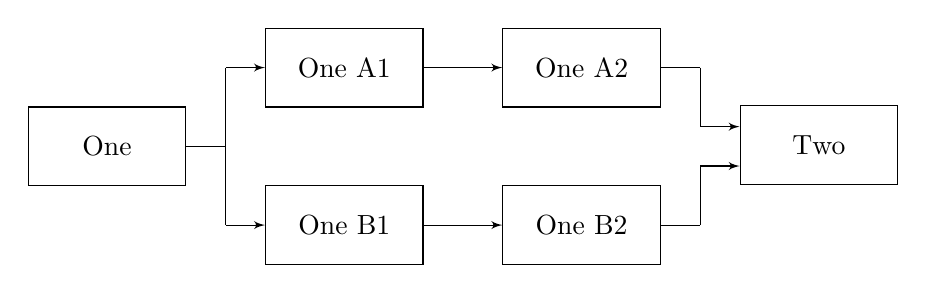
\begin{tikzpicture}[>=latex']
\tikzset{block/.style= {draw, rectangle, align=center,minimum width=2cm,minimum height=1cm},
}
\node [block]  (start) {One};
\node [coordinate, right = 0.5cm of start] (ADL){};
\node [coordinate, above = 1cm of ADL] (AUL){};
\node [coordinate, right = 0.5cm of start] (BUL){};
\node [coordinate, below = 1cm of BUL] (BDL){};
\node [block, right = 0.5cm of AUL] (A1){One A1};
\node [block, right = 0.5cm of BDL] (B1){One B1};
\node [block, right = 1cm of A1] (A2){One A2};
\node [block, right = 1cm of B1] (B2){One B2};
\node [coordinate, right = 0.5cm of A2] (AUR){};
\node [coordinate, below = 0.75cm of AUR] (ADR){};
\node [coordinate, right = 0.5cm of B2] (BDR){};
\node [coordinate, above = 0.75cm of BDR] (BUR){};
\node [coordinate, right = 0.5cm of BUR] (BEnd){};
\node [coordinate, right = 0.5cm of ADR] (AEnd){};
\node [block, above right = 0cm and 1cm of B2] (end){Two};

\path[draw, ->]
(start) -- (ADL) 
(ADL) -- (AUL)
(AUL) edge (A1)
(A1) edge (A2)
(A2) -- (AUR)
(AUR) -- (ADR)
(ADR) edge (AEnd)

(start) -- (BUL)
(BUL) -- (BDL)
(BDL) edge (B1)
(B1) edge (B2)
(B2) -- (BDR)
(BDR) -- (BUR)
(BUR) -- (BEnd)
;
\end{tikzpicture}




% ---------------------------------------------------------
\vspace{5ex}

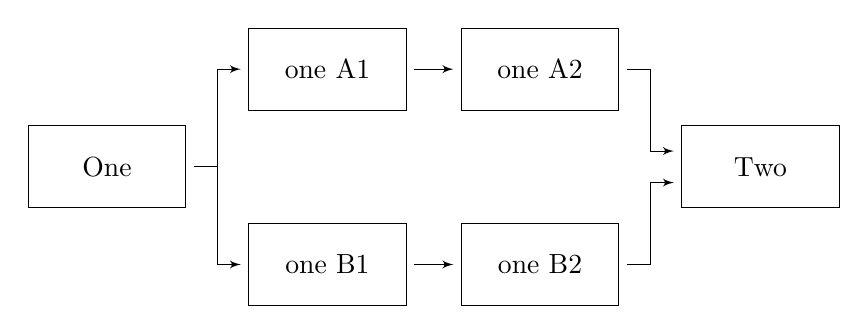
\begin{tikzpicture}[ > = latex',  node distance = 0mm and 5mm,   mynode/.style = {name = n#1, draw, minimum height = 10mm, minimum width = 20mm, inner sep = 4mm, outer sep = 1mm} ]

\node[mynode=1] {One};
	\coordinate[right = 3mm of n1] (a);
	\draw (n1) -- (a);
\node[mynode=2,above right = 0mm and 6mm of n1] {one A1};
	\draw[->] (a) |- (n2);
\node[mynode=3,right = of n2] {one A2};
	\draw[->] (n2) -- (n3);
\node[mynode=4,below right = 0mm and 6mm of n3] {Two};
	\coordinate[above left = 2mm and 3mm of n4.west] (b1);
	\draw[->] (n3) -| (b1) -- (b1 -| n4.west);
	\coordinate[below left = 2mm and 3mm of n4.west] (b2);
\node[mynode=5,below right = 0mm and 6mm of n1] {one B1};
	\draw[->] (a) |- (n5);
\node[mynode=6,right = of n5] {one B2};
	\draw[->] (n5) -- (n6);
	\draw[->] (n6) -| (b2) -- (b2 -| n4.west);
\end{tikzpicture}



% ---------------------------------------------------------
\vspace{5ex}

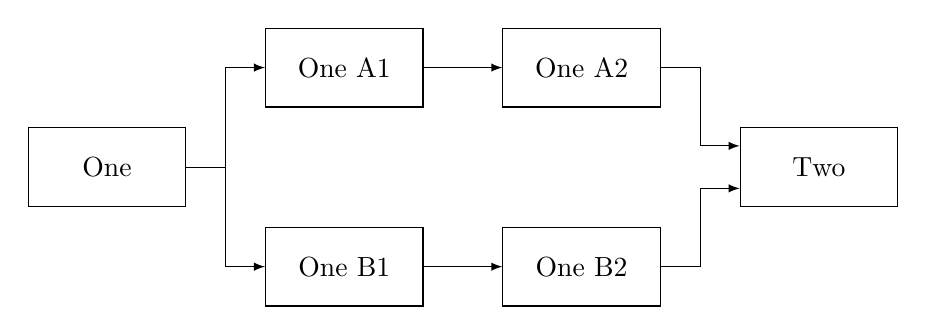
\begin{tikzpicture}[node distance=.25cm and 1cm]
\tikzset{every node/.style={rectangle, draw, minimum width=2cm, minimum height=1cm}, > = latex, }
% Nodes
\node (one) {One};
\node (a1) [above right=of one] {One A1};
\node (a2) [right=of a1] {One A2};
\node (b1) [below right=of one] {One B1};
\node (b2) [right=of b1] {One B2};
\node (two) [below right=of a2] {Two};
% Connectors
\begin{scope}[->]
\foreach \x\r in {a/165,b/195} {
	\draw (one) -| ($(one)!.5!(\x1)$) |- (\x1);
	\draw (\x1) -- (\x2);
	\draw (\x2) -| ($(\x2)!.5!(two)$) |- (two.\r);  }
\end{scope}
\end{tikzpicture}



% ---------------------------------------------------------
\vspace{5ex}
from https://tex.stackexchange.com/questions/71478/how-to-center-one-node-exactly-between-two-others-with-tikz website.

\scalebox{4}{
\begin{tikzpicture}[text height=2ex]
\node (a) {a};
\node (c) [right of=a] {c};
\node (b) at ($(a)!0.5!(c)$) {b};
\end{tikzpicture}    }



% ---------------------------------------------------------
\vspace{5ex}
from https://tex.stackexchange.com/questions/123671/manual-automatic-line-breaks-and-text-alignment-in-tikz-nodes 

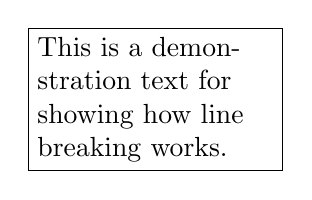
\begin{tikzpicture}
\node (example-textwidth-2) [draw, text width=3cm]{This is a demonstration text for showing how line breaking works.};
\end{tikzpicture}

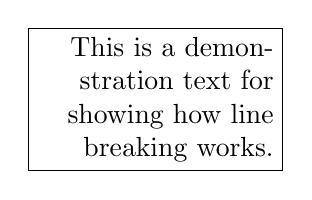
\begin{tikzpicture}
\node (example-textwidth-2) [draw, text width=3cm, align=right]{This is a demonstration text for showing how line breaking works.};
\end{tikzpicture}

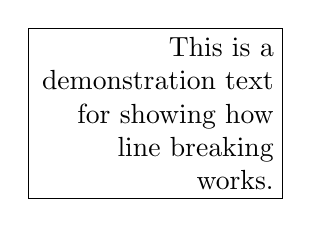
\begin{tikzpicture}
\node (example-textwidth-2) [draw, text width=3cm, align=flush right]{This is a demonstration text for showing how line breaking works.};
\end{tikzpicture}



% ---------------------------------------------------------
\vspace{5ex}
from https://texample.net/tikz/examples/control-system-principles/ website.

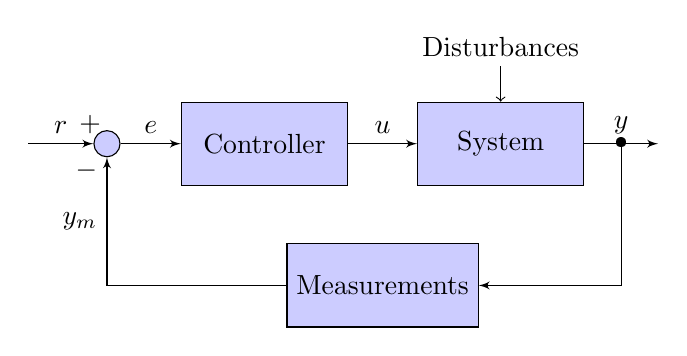
\begin{tikzpicture}[auto, node distance=2cm,> =latex']
\tikzstyle{block} = [draw, fill=blue!20, rectangle, minimum height=3em, minimum width=6em]
\tikzstyle{sum} = [draw, fill=blue!20, circle, node distance=1cm]
\tikzstyle{input} = [coordinate]
\tikzstyle{output} = [coordinate]
\tikzstyle{pinstyle} = [pin edge={to-,thin,black}]

\node [input, name=input] {};
\node [sum, right of=input] (sum) {};
	\draw [draw,->] (input) -- node{$r$} node[pos=0.95]{$+$} (sum);
\node [block, right of=sum] (controller) {Controller};
	\draw [->] (sum) -- node{$e$} (controller);
\node [block, right of=controller, pin={[pinstyle]above:Disturbances}, node distance=3cm] (system) {System};
	\draw [->] (controller) -- node[name=u]{$u$} (system);
\node [output, right of=system] (output) {};
	\draw [->] (system) -- node[name=y]{$y$} (output);
%\coordinate [below of=u] (unity);
%	\draw [->] (y) |- (unity) -| node[pos=0.95]{$-$} (sum);
\node [block, below of=u] (measurements) {Measurements};
	\draw [->] (y) |- (measurements);
	\draw [->] (measurements) -| node[pos=0.95]{$-$} node[near end]{$y_m$} (sum);
	draw \node at (y.south) {\textbullet};
\end{tikzpicture}



% ---------------------------------------------------------
\vspace{5ex}
from https://tex.stackexchange.com/questions/175969/block-diagrams-using-tikz website.

%\begin{figure}[!htb]
%\centering
\begin{tikzpicture}[auto, node distance=2cm,>=latex']
\tikzset{block/.style={draw, fill=white, rectangle, minimum height=3em, minimum width=3em},   tmp/.style={coordinate},     sum/.style={draw, fill=white, circle, node distance=1cm},    input/.style={coordinate}, output/.style={coordinate},    pinstyle/.style={pin edge={to-,thin,black}}   }
\node [input, name=rinput] (rinput) {};
\node [sum, right of=rinput] (sum1) {};
\node [block, right of=sum1] (kp) {$k_{p\beta}$};
\node [block, above of=kp,node distance=1.3cm] (ki){$\frac{k_{i\beta}}{s}$};
\node [block, below of=kp,node distance=1.3cm] (kd) {$sk_{d\beta}$};
\node [sum, right of=kp,node distance=2cm] (sum2) {};
\node [block, above = 2cm of sum2](extra){$\frac{1}{\alpha_{\beta2}}$};  %
\node [block, right of=sum2,node distance=2cm] (system) 
{$\frac{a_{\beta 2}}{s+a_{\beta 1}}$};
\node [output, right of=system, node distance=2cm] (output) {};
\node [tmp, below of=kp] (tmp1){$H(s)$};

\draw [->] (rinput) -- node{$R(s)$} (sum1);
\draw [->] (sum1) -- node[name=es,anchor=north]{$E(s)$} (kp);
\draw [->] (kp) -- (sum2);
\draw [->] (sum2) -- node{$U(s)$} (system);
\draw [->] (system) -- node [name=y] {$Y(s)$}(output);
\draw [->] (es) |- (kd);  
\draw [->] (kd) -| (sum2);
\draw [->] (es) |- (ki);  
\draw [->] (ki) -| (sum2);
\draw [->] (y) |- (tmp1)-| node[pos=0.95] {$-$} (sum1);
\draw [->] (extra)--(sum2);
\draw [->] ($(0,1.5cm)+(extra)$) node[above]{$d_{\beta 2}$} -- (extra);
\end{tikzpicture}
%\caption{A PID Control System} \label{fig6_10}
%\end{figure}



% ---------------------------------------------------------
\vspace{5ex}
Using \texttt{schemablock} package (terms in French):

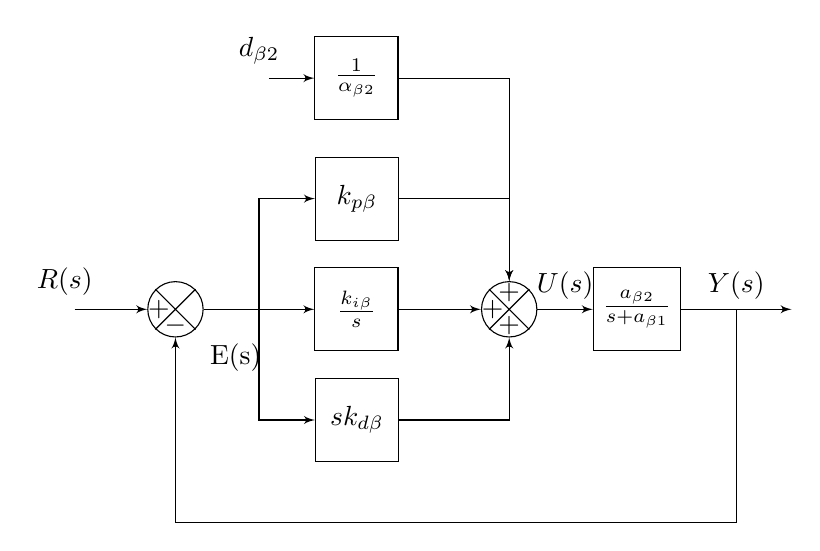
\begin{tikzpicture}
\sbEntree{E}                      
\sbNomLien[1]{E}{$R(s)$}
\sbComp{C1}{E}
\sbRelier{E}{C1}  
\sbBlocL[4]{Int}{$\frac{k_{i\beta}}{s}$}{C1}
\node[below right=0.25em of C1]{E(s)};
\sbDecaleNoeudy[4]{Int}{Der}
\sbDecaleNoeudy[-4]{Int}{Prop}
\sbBloc[-1.5]{Der}{$sk_{d\beta}$}{Der}  \sbRelieryx{C1-Int}{Der}
\sbBloc[-1.5]{Prop}{$k_{p\beta}$}{Prop}        \sbRelieryx{C1-Int}{Prop}
\sbCompSum{Somme}{Int}{+}{+}{+}{ }
\sbRelier{Int}{Somme}  
\sbRelierxy{Prop}{Somme}
\sbRelierxy{Der}{Somme}
\sbBloc{F1}{$\frac{a_{\beta 2}}{s+a_{\beta 1}}$}{Somme}
\sbRelier[$U(s)$]{Somme}{F1} 
\sbSortie[4]{S}{F1}               \sbRelier[$Y(s)$]{F1}{S}               
\sbRenvoi[7]{F1-S}{C1}{}          
\sbDecaleNoeudy[-8]{C1-Int}{E2}
\sbBlocL{F2}{$\frac{1}{\alpha_{\beta2}}$}{E2}
\sbNomLien[1]{E2}{$d_{\beta 2}$}
\sbRelierxy{F2}{Somme}
\end{tikzpicture}




% ---------------------------------------------------------
\vspace{5ex}
Using \texttt{schemablock} package (terms in English):

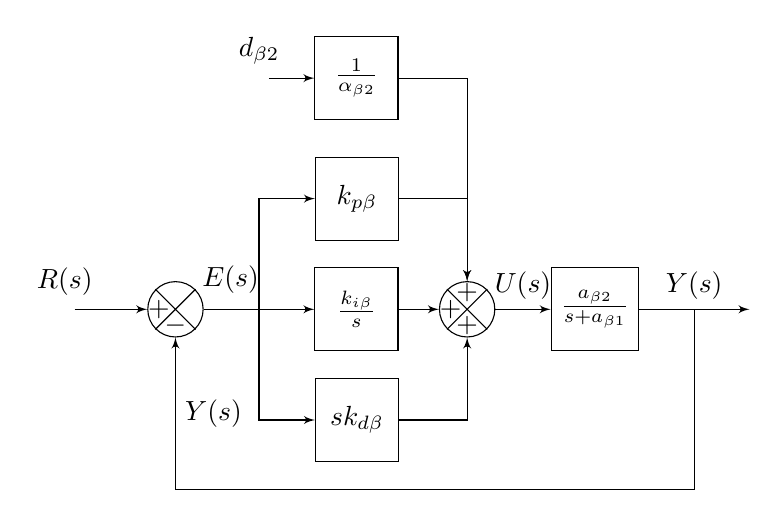
\begin{tikzpicture}
\bXInput{r}    \bXLinkName[1]{r}{$R(s)$}
\bXComp{C1}{r}    \bXLink{r}{C1}  
\bXBlocL[4]{Int}{$\frac{k_{i\beta}}{s}$}{C1}
\node[above right=-0.5em and -0.1em of C1]{$E(s)$};
\bXNodeShifty[4]{Int}{Der}
\bXBloc[-1.5]{Der}{$sk_{d\beta}$}{Der}    \bXLinkyx{C1-Int}{Der}
\bXNodeShifty[-4]{Int}{Prop} 
\bXBloc[-1.5]{Prop}{$k_{p\beta}$}{Prop}    \bXLinkyx{C1-Int}{Prop}
\bXCompSum{Sum}{Int}{+}{+}{+}{ }
\bXLink{Int}{Sum}    \bXLinkxy{Prop}{Sum}    \bXLinkxy{Der}{Sum}
\bXBloc{F1}{$\frac{a_{\beta 2}}{s+a_{\beta 1}}$}{Sum}    \bXLink[$U(s)$]{Sum}{F1} 
\bXOutput[4]{S}{F1}    \bXLink[$Y(s)$]{F1}{S}               
\bXReturn[7]{F1-S}{C1}{$Y(s)$}          
\bXNodeShifty[-8]{C1-Int}{E2}
\bXBlocL{F2}{$\frac{1}{\alpha_{\beta2}}$}{E2}
\bXLinkName[1]{E2}{$d_{\beta 2}$}    \bXLinkxy{F2}{Sum}
\end{tikzpicture}



% ---------------------------------------------------------
\vspace{5ex}
from https://tex.stackexchange.com/questions/206866/a-block-diagram-in-tikz website.

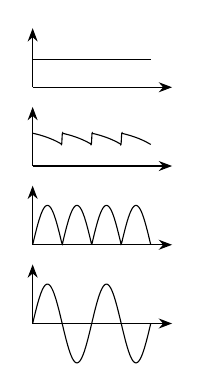
\begin{tikzpicture}[> = Stealth] % use arrows.meta tikzlibrary
	\tikzset{ function/.pic = { \tikzset{x=1.5cm/720, y=1cm/2} \draw [->] (0,0) -- (850,0); \draw [->] (0,0) -- (0,1.5); \draw  plot [domain=0:720, samples=180, smooth] (\x, {#1});  }  }

	\path (0,0)  pic {function={sin(\x)}};
	\path (0,1)  pic {function={abs(sin(\x))}};
	\path (0,2)  pic {function={1-exp(mod(\x,180)/180)/6}};
	\path (0,3)  pic {function={1/sqrt(2)}};
\end{tikzpicture}



% ---------------------------------------------------------
\vspace{5ex}
from https://tex.stackexchange.com/questions/206866/a-block-diagram-in-tikz website.

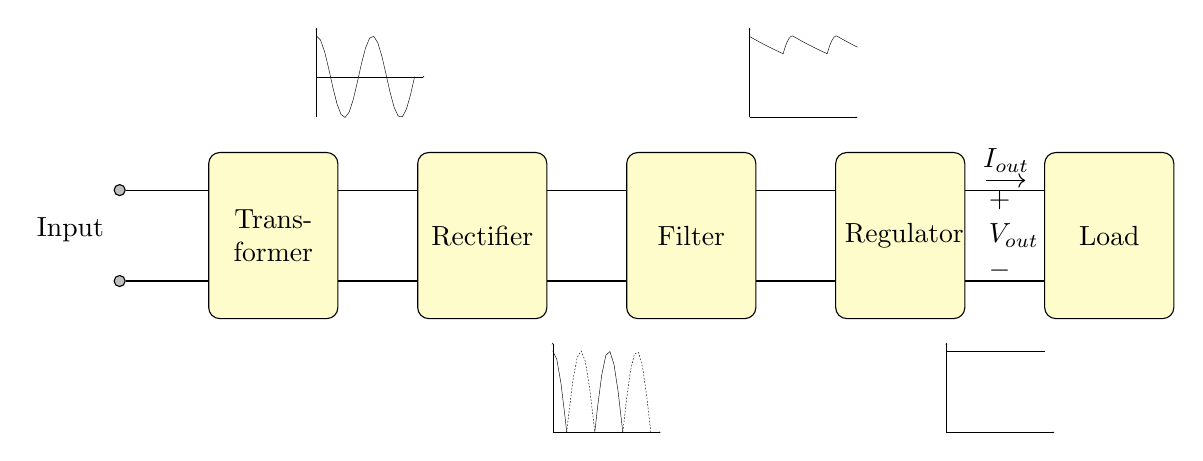
\begin{tikzpicture}[]
\tikzset{  block/.style = {rectangle, draw, fill=yellow!20, text width=4em, text centered, rounded corners, minimum height=6em},    line/.style = {draw, -latex'},    io/.style={draw, circle, inner sep=0pt, minimum size=4pt, fill=gray!50}  }

\tikzset{
	mysine/.pic={ \begin{axis}    [axis x line=center, ticks=none, axis y line=left, enlargelimits=upper]    \addplot[ thick, domain=-pi:6*pi] {-2*sin(deg(0.5*x))};    \end{axis}  }, 
	reti/.pic={ \begin{axis}    [axis x line=center, ymin=0,ticks=none, axis y line=left, enlargelimits=upper]    \addplot[thick, domain=-pi:6*pi] {-2*sin(deg(0.5*x))};    \addplot[dashed, thick, domain=-pi:6*pi] { 2*sin(deg(0.5*x))};    \end{axis}  }, 
	filted/.pic={ \def\arch{1.7*pi/3}    \begin{axis}    [xmin=-3,xmax=11, ymin=0, ticks=none, axis x line=center, axis y line=left, enlargelimits=upper]    \foreach \i/\j/\k in {-1/0/1,1/2/3,3/4/5,5/6/7} {  \addplot[thick, domain=\i*pi:{\j*pi+\arch}] {2*e^(-0.05*(x-\i*pi)};    \addplot[thick, smooth, domain={\j*pi+\arch}:\k*pi] {2*sin(deg(0.5*x))};    \addplot [thick, domain={\j*pi+\arch}:\k*pi, smooth] {-2*sin(deg(0.5*x))};   }    \end{axis}  },
	dc/.pic={ \begin{axis}    [xmin=0, xmax=11, ymin=0, axis x line=center, ticks=none, axis y line=left, enlargelimits=upper]    \addplot[thick, domain=0:11] {2};    \end{axis}  },        }

	\node  (in1) [above=1cm,io, label={[yshift=-0.5cm]left:Input}]{};
	\node  (in2) [below=1cm of in1, io]{};
	\node (out1) [right= 13cm of in1]{};
	\node (out2) [right= 13cm of in2]{};
	\draw (in1)--node[pos=0.86,above=3pt]{$I_{out}$}(out1);
	\draw (in2)--(out2);
	\path (in1)--node[pos=0.5](a){}(in2)
		node[block,right=1cm of a](t){Trans-\\former}
		node[block,right=1cm of t](r){Rectifier}
		node[block,right=1cm of r](f){Filter} 
		node[block,right=1cm of f](re){Regulator}
		node[block,right=1cm of re](l){Load}  ;
	\draw[->] (11,1.2)--+(0.5,0);
	\node[above right=0.2cm and 1cm] at (re){$+$};
	\node[right=1cm] at (re){$V_{out}$};
	\node[below right=0.2cm and 1cm] at (re){$-$};
	\pic at (2.5,2) [scale=0.2]{mysine};
	\pic at (5.5,-2) [scale=0.2]{reti};
	\pic at (8,2) [scale=0.2]{filted};
	\pic at (10.5,-2) [scale=0.2]{dc};
\end{tikzpicture}



% ---------------------------------------------------------
\vspace{5ex}
from https://tex.stackexchange.com/questions/237765/block-diagram-using-tikz?rq=1 website.

\begin{tikzpicture}[block1/.style={draw, minimum width=3cm, minimum height=1.8cm},    block2/.style={draw, minimum width=1cm, minimum height=.8cm},    > =Stealth]
\node[block1,label=above:lol] (b1) {lol};
\node[block1, right=5cm of b1] (b2) {lol2};
\draw[->] ([yshift=3mm]b1.east) -- node[above] {c} ([yshift=3mm]b2.west);
\path ([yshift=-3mm]b1.center) -- ([yshift=-3mm]b2.center) node [midway,block2] (b3) {lol3};
\draw[->] ([yshift=-3mm]b1.east) -- node[below]{a} (b3.west);
%\draw[<-] ([yshift=-3mm]b2.west)--node[below]{b} (b3.east);
\draw[->] (b3.east) -- node[below]{b} ([yshift=-3mm]b2.west);
\draw[->] (b2.east) --++(0:1cm) node[right]{thanks!};
\end{tikzpicture}



% ---------------------------------------------------------
\vspace{5ex}
from https://tex.stackexchange.com/questions/166838/block-diagram-with-dsp-tikz-for-adaptive-feedback-cancellation

In a comment, some problem with cut labels was mentioned when including the figure from an external file. In this case, I'd suggest you to use the \verb|standalone| documentclass to produce your image as a separate pdf file that then can be easily included in your document using the standard \verb|\includegraphics| mechanism from graphicx; you can use the border option for standalone to control the padding around your figure, in case it is required:

%\begin{tikzpicture}
%% Blocks and nodes
%\node[dspnodeopen,dsp/label=below] (ns) {$v(t)$}; 
%\node[left=of ns,fill=gray,circle,draw] (mic) {};
%\draw ([yshift=8pt]mic.east) -- ([yshift=-8pt]mic.east);
%\node[dspadder,left=of mic,left=1.5cm,label={above right:$-$},label={below right:$+$}] (add) {};
%\node[coordinate,left=of add,left=2.35cm] (fp1) {};
%\node[dspfilter,minimum height=2cm,above=of fp1,above=1.5cm] (gain) {$G$};
%\node[coordinate,above=of gain,above=1.5cm] (fp2) {};
%\node[dspnodefull,right=of fp2,right=2.55cm] (adnode) {$u(t)$};
%\node[dspfilter,minimum height=2cm,right=of gain,right=1.15cm] (adfilt) {$\hat{F}$};
%\node[draw,right= 4cm of fp2,fill=gray,trapezium,shape border rotate=90,shape border uses incircle] (ls) {};
%\draw ([yshift=-10pt]ls.west) -- ([yshift=10pt]ls.west);
%\node[dspfilter,minimum height=2cm,right=of gain,right=4cm] (feedback) {F};
%\node[dspnodefull,left=of add] (afupd1) {};
%\node[coordinate,above=of afupd1,above=1cm] (afupd2) {};
%\coordinate (aux) at ([yshift=-4pt]adfilt.center);
%% Connections
%\draw[dspconn] (ns) -- (mic);
%\draw[dspconn] (mic) -- node[midway,below=0.09cm] {$y(t)$} (add);
%\draw[dspline] (add) -- node[midway,below] {$d[t,\hat{\mathbf{f}}(t)]$} (fp1);
%\draw[dspline,dashed] (afupd1) -- (afupd2);
%\draw[dspconn,dashed] (afupd2) -- ( $ (afupd2)!2.7cm!(aux) $ );
%\draw[dspconn] (fp1) -- (gain);
%\draw[dspline] (gain) -- (fp2);
%\draw[dspline] (fp2) -- (adnode);
%\draw[dspconn] (adnode) -- (ls);
%\draw[dspconn] (adnode) -- (adfilt);
%\draw[dspconn] (adfilt) -- node[midway,right] {$\hat{y}[t |\hat{\mathbf{f}}(t)]$} (add);
%\draw[dspconn] (ls) to[out=0,in=90] (feedback);
%\draw[dspconn] (feedback) to[out=-90,in=30] ([yshift=3pt]mic.east);
%\end{tikzpicture}



%% ---------------------------------------------------------
%\vspace{5ex}
%
%\begin{tikzpicture}
%\renewcommand{\dspfilterwidth}{8mm}
%\newcommand{\dspfilterheight}{1.8cm}
%\tikzset{dspfilter/.append style = {minimum height=\dspfilterheight}}
%\newcommand{\dspvspace}{1.2cm}
%
%% Blocks and nodes
%\node[dspnodeopen, dsp/label=below] (ns) {$v(t)$}; 
%\node[left=of ns, fill=gray, circle, draw] (mic) {};
%\draw ([yshift=8pt] mic.east) -- ([yshift=-8pt] mic.east);
%\node[dspadder, left=of mic, left=2.35cm, label={above right:$-$}, label={below right:$+$}] (add) {};
%\node[coordinate, left=of add, left=1.8cm] (fp1) {};
%\node[dspfilter, above=of fp1, above=\dspvspace] (gain) {$G$};
%\node[coordinate, above=of gain, above=\dspvspace] (fp2) {$fp2$};
%\node[dspnodefull, above=of add, above=2*\dspvspace+\dspfilterheight-0.5*\dspoperatordiameter-\dspblocklinewidth] (adnode) {$u(t)$};
%\node[dspfilter, above=of add, above=\dspvspace-0.5*\dspoperatordiameter] (adfilt) {$\hat{F}$};
%\node[draw, above=of mic, above=2*\dspvspace+\dspfilterheight-\dspblocklinewidth-0.4cm, fill=gray, trapezium, shape border rotate=90, shape border uses incircle] (ls) {};
%\draw ([yshift=-10pt] ls.west) -- ([yshift=10pt] ls.west);
%\node[dspfilter, above=of ns, above=\dspvspace] (feedback) {$F$};
%\node[dspnodefull, left=of add, left=0.8cm] (afupd1) {};
%\node[coordinate, above=of afupd1, above=\dspvspace] (afupd2) {};
%\coordinate (aux) at (adfilt.center);
%% Connections
%\draw[dspconn] (ns) -- (mic);
%\draw[dspconn] (mic) -- node[midway,below=0.09cm] {$y(t)$} (add);
%\draw[dspline] (add) -- node[midway,below] {$d[t,\hat{\mathbf{f}}(t)]$} (fp1);
%\draw[dspline,dashed] (afupd1) -- (afupd2);
%\draw[dspconn,dashed] (afupd2) -- ( $ (afupd2)!3cm!(aux) $ );
%\draw[dspconn] (fp1) -- (gain);
%\draw[dspline] (gain) -- (fp2);
%\draw[dspline] (fp2) -- (adnode);
%\draw[dspconn] (adnode) -- (ls);
%\draw[dspconn] (adnode) -- (adfilt);
%\draw[dspconn] (adfilt) -- node[midway,right] {$\hat{y}[t |\hat{\mathbf{f}}(t)]$} (add);
%\draw[dspconn] (ls) to[out=0,in=90] (feedback);
%\draw[dspconn] (feedback) to[out=-90,in=30] ([yshift=3pt]mic.east);
%\end{tikzpicture}



% ---------------------------------------------------------
\vspace{5ex}
from https://tex.stackexchange.com/questions/200235/is-there-a-predefined-bandpass-filter-block-in-tikz

\newcommand{\cross}[1] {  \draw[thick] (#1) circle (12pt);    \draw[rotate=45,line width=0.5pt]   (#1)  +(0,-12pt) -- +(0,12pt);    \draw[rotate=-45,line width=0.5pt]  (#1)  +(0,-12pt) -- +(0,12pt);  }

\newcommand{\BPF}[2] {  \begin{scope}[transform shape,rotate=#2]    \draw[thick] (#1)node[](a){} +(-12pt,-12pt) rectangle +(12pt,12pt);    \draw (a) +(-8pt,0) to[bend left] +(0,0) edge[bend right] +(8pt,0);    \draw ([yshift=5pt]a) +(-8pt,0) to[bend left] +(0,0) to[bend right] +(8pt,0);    \draw ([yshift=-5pt]a) +(-8pt,0) to[bend left] +(0,0) edge[bend right] +(8pt,0);    \draw[rotate=20] ([yshift=5pt]a) +(-4pt,0) -- +(7pt,0);    \draw[rotate=20] ([yshift=-5pt]a) +(-7pt,0) -- +(4pt,0);    \end{scope}    }


	
\begin{circuitikz}
\tikzset{ar/.style={-latex,shorten >=-1pt, shorten <=-1pt}}
\path (4,0) node[above=1pt](lo){LO}  to[sV] node[pos=0,inner sep=0pt](b){} (4,2);
\draw (0,3)  node[buffer,scale=0.8](buf){}  node[above =0.8 cm]{LNA};
\path (1,3) to[sV,color=white,name=bp]  node[pos=0,inner sep=0pt](d){}  node[above left=0.8cm and 0.5cm]{BPF} (3,3);
\BPF{bp}{0}
\path (4,2) to[sV, color=white, name=M1]  node[midway] {Mixer}  (4,4);
\cross{M1}
\draw[]  (-1,3)  node[antenna, xscale=-1](A){}  --  (buf.in);
\draw[ar]  (bp) -- (M1);
\draw[ar]  (buf.out) -- (bp);
\draw[ar]  (b) -- (M1);
\draw[ar]  (M1) -- +(2,0);
\end{circuitikz}



%% ---------------------------------------------------------
%\vspace{5ex}
%from https://tex.stackexchange.com/questions/127663/drawing-control-diagram-in-latex
%
%\tikzstyle{decision} = [diamond, draw, fill=blue!20,text width=4.5em, text badly centered, node distance=3cm, inner sep=0pt]
%\tikzstyle{block} = [rectangle, draw, fill=blue!20,text width=5em, text centered, minimum height=4em]
%\tikzstyle{cloud} = [draw, ellipse,fill=red!20, node distance=3cm,minimum height=2em]
%\tikzstyle{line} = [draw, -stealth, thick]
%\tikzstyle{input} = [coordinate]
%\tikzstyle{output} = [coordinfor future referenceate]
%\tikzstyle{pinstyle} = [pin edge={to-,thin,black}]
%
%\begin{tikzpicture}[auto,node distance =3cm,>=latex',
%path/.style={->, >=stealth, postaction = decorate},
%decoration={markings, mark = at position 1cm with {\arrow[black]{stealth}}
%}]
%
%% Place nodes
%\node [input, name = input]{Input command};
%\node [block, right of = input] (control) {Controller $C(\theta_c)$};
%\node [block, right of = control](plant){Plant $G(\theta^*$)};
%\node [right of = plant] (output){y};
%\node [block, below of = plant][yshift=1.25cm] (O_p_e) {Online Parameter Estimator};
%\node [block, below of = O_p_e] [yshift=1cm](C_c_p) {Calculation of control parameters};
%\draw[draw,->] ([yshift=-1em]input) -- node [above of = input, node distance = 1em]{Input} ([yshift=-1em]control.west);
%\draw [->] (control) -- node {$u$} (plant);
%\draw [->] (O_p_e) -- node {$\theta(t)$}(C_c_p);
%\draw [->] (control) -- (4.5,0) |- node {} (O_p_e);
%\draw [->] (C_c_p) -| node {$\theta_c(t)$} (control);
%\path[line] (plant) -- (output);
%\draw [->] (plant) -- (7.5,0) |- node {} (O_p_e);
%\draw [->] (plant) -- (7.5,0) -- (7.5,1) -| (0.5,1) |- node {} ([yshift = -0.2cm]control.north west);
%\end{tikzpicture}



%% ---------------------------------------------------------
%\vspace{5ex}
%
%\makeatletter
%\dspdeclareoperator{dspvoidshapeadder}{
%	% Coordinate offset for the plus
%	\pgfutil@tempdima=\radius
%	\pgfutil@tempdima=0.55\pgfutil@tempdima
%	\pgfusepathqstroke
%}
%\makeatother
%\begin{tikzpicture}
%\tikzset{
%	vdspadder/.style={ shape=dspvoidshapeadder, line cap=rect, 		line join=rect, line width=\dspblocklinewidth, minimum size=\dspoperatordiameter, label={185:$+$}, label={265:$-$}  },
%	vadspadder/.style={ shape=dspvoidshapeadder, line cap=rect, line join=rect, line width=\dspblocklinewidth, minimum size=\dspoperatordiameter, label=below right:$-$, label=above right:$+$ }  }
%
%% the nodes
%\matrix[row sep=10mm, column sep=10mm] 
%{	& \node[vdspadder] (g1) {}; &  & \node[dspsquare] (g2) {$k_{\text{pr}}$}; & \node[dspfilter,text width=2cm] (g3) {Yaw Model}; \\
%\node[dspnodeopen,label=above left:$r_{des}$] (g4) {}; &  &  &  & \node[dspfilter,text width=2cm,text height=1.5em,text depth=2em] (g5) {Adaptation \\Law}; & \node[vadspadder] (g6) {};  \\ 
%& \node[vdspadder] (g7) {}; & \node[dspsquare] (g8) {$k_{\text{pr}}$}; & \node[dspsquare] (g9) {$K$}; & \node[dspfilter,text width=2cm] (g10) {Yaw Plant}; \\
%};
%% the connections
%\draw (g4) -- +(-20pt,0);
%\draw[dspconn] (g4) -- (g5);
%\draw[dspconn] (g4) |- coordinate[pos=0.85] (aux4) (g1);
%\draw[dspconn] (g1) -- (g2);
%\draw[dspconn] (g2) -- node[above] {$\delta_{\textrm{mod}}$} (g3);
%\draw[dspconn] (g3) -| node[dspnodeopen,pos=0.25] (aux1) {} (g6) node[label=right:$r_{\textrm{mod}}$,pos=0.75] {};
%\draw[dspconn] (g6) -- node[auto,swap] {$e$} (g5);
%\draw[dspconn] (aux1) -- +(0,-30pt) -| (g1);
%\draw[dspconn] (g4) |- (g7);
%\draw[dspconn] (g7) -- (g8);
%\draw[dspconn] (g8) -- (g9);
%\draw[dspconn] (g9) -- node[below,pos=0.25] {$\delta$} (g10);
%\draw[dspconn] (g10) -| node[dspnodeopen,pos=0.25] (aux2) {} (g6) node[label=right:$r$,pos=0.75] {};
%\draw[dspconn] (aux2) |- (g5.-20);
%\draw[dspconn] (aux2) |- +(0,-30pt) -| (g7);
%\draw (g5.270) |- +(0,-22pt) -| (g9);
%\draw[dspconn] (g9.south) -- +(0,-10pt);
%
%% the fitting dashed nodes
%\coordinate (aux3) at ([yshift=-20pt]aux1);
%\node[draw,inner xsep=10pt,inner ysep=20pt,dashed,fit=(aux4) (aux3),label=above:{Closed-Loop Yaw Model}] {};
%\node[draw,inner xsep=20pt,inner ysep=12pt,dashed,fit=(g8) (g9),label=above:{Yaw Rate Controller}] {};
%\end{tikzpicture}



% ---------------------------------------------------------
\vspace{5ex}
\noindent from https://www.overleaf.com/learn/latex/LaTeX\_Graphics\_using\_TikZ:\_A \_Tutorial\_for\_Beginners\_(Part\_1)\%E2\%80\%94Basic\_Drawing

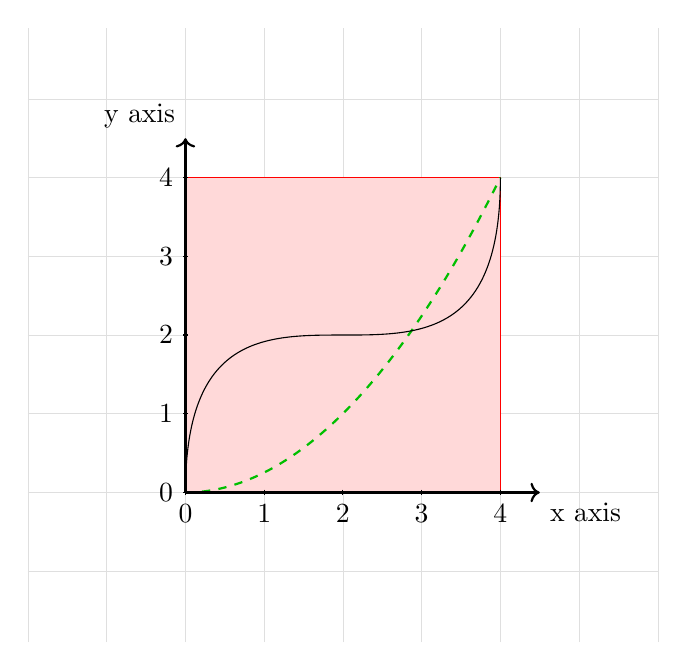
\begin{tikzpicture}
\draw[step=1cm,gray!25,very thin] (-2,-1.9) grid (6,5.9);
\filldraw[fill=red!15!white, draw=red] (0,0) rectangle (4,4);
\draw[green!75!black,dashed,thick,] (0,0) parabola (4,4);
\draw[] (0,0) .. controls (0,4) and (4,0) .. (4,4);
\draw[thick,->] (0,0) -- (4.5,0) node[anchor=north west] {x axis};
\draw[thick,->] (0,0) -- (0,4.5) node[anchor=south east] {y axis};
\foreach \x in {0,1,2,3,4}
\draw (\x cm,1pt) -- (\x cm,-1pt) node[anchor=north] {$\x$};
\foreach \y in {0,1,2,3,4}
\draw (1pt,\y cm) -- (-1pt,\y cm) node[anchor=east] {$\y$};
\end{tikzpicture}

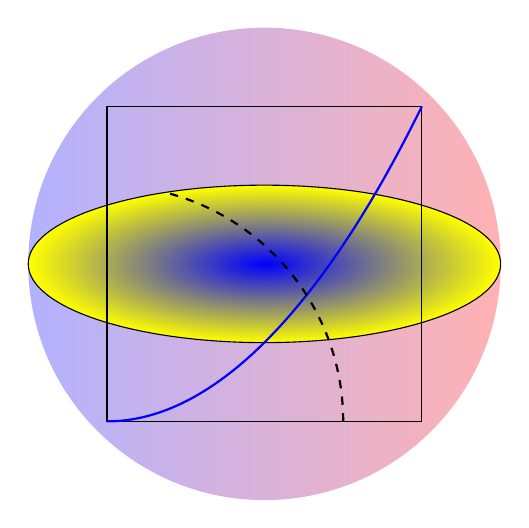
\begin{tikzpicture}
\shade[left color=blue!30,right color=red!30] (2,2) circle (3cm);
\shadedraw[inner color=blue,outer color=yellow, draw=black] (2,2) ellipse (3cm and 1cm);
\draw (0,0) -- (4,0) -- (4,4) -- (0,4) -- cycle;
\draw[blue,thick,] (0,0) parabola (4,4);
\draw[black,dashed,thick] (3,0) arc (0:75:3cm);
\end{tikzpicture}



% ---------------------------------------------------------
\vspace{5ex}
from https://www.overleaf.com/learn/latex/LaTeX\_Graphics\_using\_TikZ:\_A \_Tutorial\_for\_Beginners\_(Part\_3)\%E2\%80\%94Creating\_Flowcharts

\begin{figure}[h!] \centering
	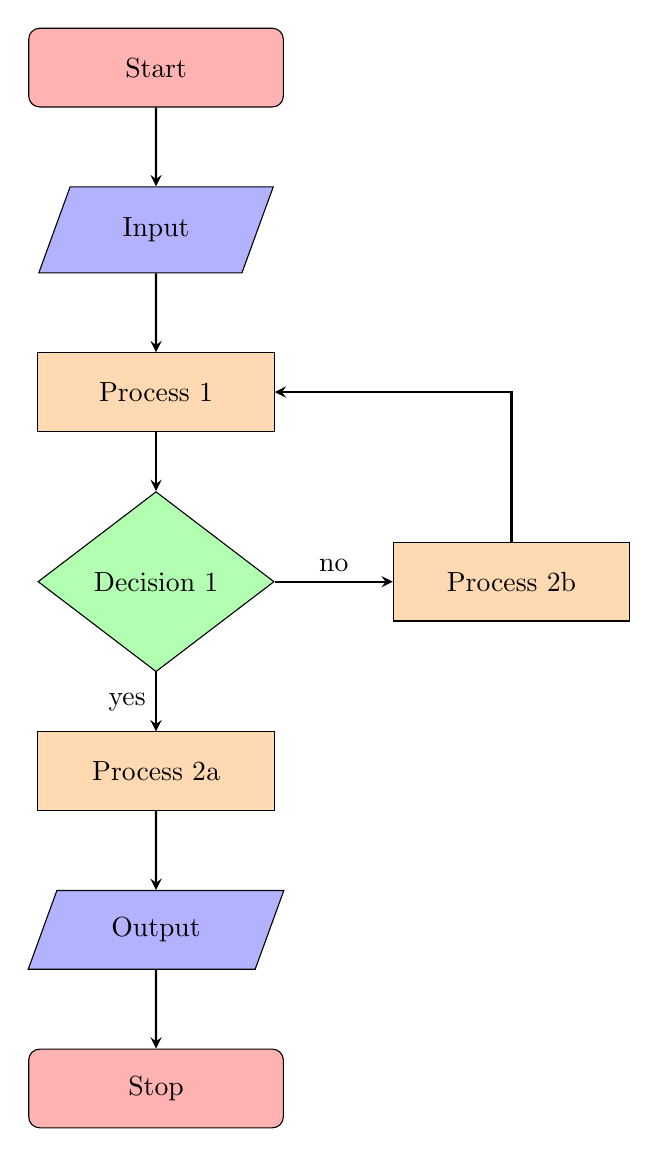
\begin{tikzpicture}[node distance=1cm]
	\tikzstyle{startstop} = [rectangle, rounded corners, minimum width=3cm, minimum height=1cm,text centered, text width=3cm, draw=black, fill=red!30]
	\tikzstyle{io} = [trapezium, trapezium left angle=70, trapezium right angle=110, minimum width=3cm, minimum height=1cm, text centered, draw=black, fill=blue!30]
	\tikzstyle{process} = [rectangle, minimum width=3cm, minimum height=1cm, text centered, draw=black, fill=orange!30]
	\tikzstyle{decision} = [diamond, minimum width=3cm, minimum height=1cm, text centered, draw=black, fill=green!30]
	\tikzstyle{arrow} = [thick,->,>=stealth]
	
	\node (start) [startstop] {Start};
	\node (in1) [io, below=of start] {Input};
	\node (pro1) [process, below=of in1] {Process 1};
	\node (dec1) [decision, below=of pro1, yshift=0.25cm] {Decision 1};
	\node (pro2a) [process, below=of dec1, yshift=0.25cm] {Process 2a};
	\node (pro2b) [process, right=of dec1, xshift=0.5cm] {Process 2b};
	\node (out1) [io, below=of pro2a] {Output};
	\node (stop) [startstop, below=of out1] {Stop};
	
	\draw [arrow] (start) -- (in1);
	\draw [arrow] (in1) -- (pro1);
	\draw [arrow] (pro1) -- (dec1);
	\draw [arrow] (dec1) -- node[anchor=east] {yes} (pro2a);
	\draw [arrow] (dec1) -- node[anchor=south] {no} (pro2b);
	\draw [arrow] (pro2b) |- (pro1);
	\draw [arrow] (pro2a) -- (out1);
	\draw [arrow] (out1) -- (stop);
	\end{tikzpicture}
	\caption{flowchart}
\end{figure}



% ---------------------------------------------------------
\vspace{5ex}

from https://tex.stackexchange.com/questions/354401/how-to-draw-a-vector-diagram-with-tikz-datavisualization


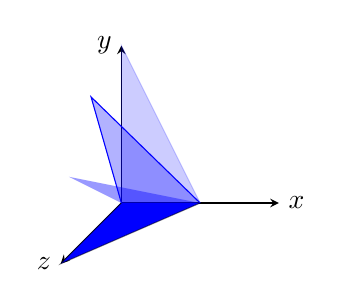
\begin{tikzpicture}[>=stealth]
\draw [->] (0,0,0) -- (2,0,0) node [at end, right] {$x$};
\draw [->] (0,0,0) -- (0,2,0) node [at end, left] {$y$};
\draw [->] (0,0,0) -- (0,0,2) node [at end, left] {$z$};

\filldraw [blue, opacity=0.2, rotate around x=0] (0,0,0) -- (0,2,0) -- (1,0,0);
\filldraw [blue,fill opacity=0.3, rotate around x=30] (0,0,0) -- (0,2,0) -- (1,0,0);
\fill [blue,fill opacity=0.4, rotate around x=60] (0,0,0) -- (0,2,0) -- (1,0,0);
\draw [fill=blue,draw opacity=0.5, rotate around x=90] (0,0,0) -- (0,2,0) -- (1,0,0);
\end{tikzpicture}



% ---------------------------------------------------------
\vspace{5ex}

from https://tex.stackexchange.com/questions/110209/high-level-digital-design-in-tikz

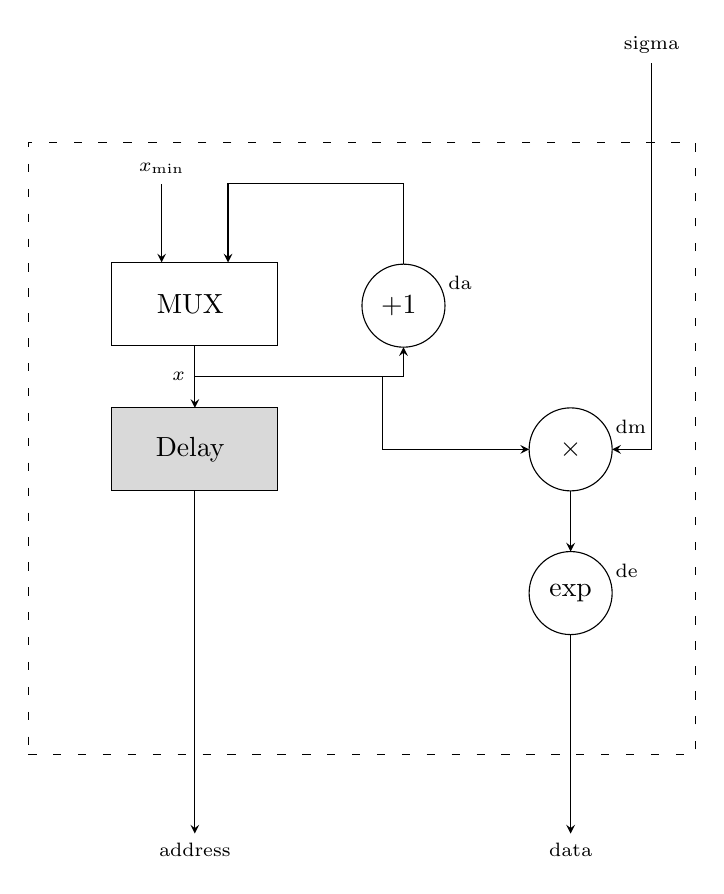
\begin{tikzpicture}[every label/.style={font=\scriptsize},>=stealth]
\tikzset{multiplexor/.style={rectangle, draw, align=center, minimum width = 6em, minimum height = 3em}}
\tikzset{register/.style={multiplexor,fill=gray!30}}
\tikzset{operation/.style={circle, draw, align=center, minimum size=3em,outer sep=0pt}}
\tikzset{port/.style={pin edge={to->,thin,black}}}

% code from Azetina:
% https://tex.stackexchange.com/questions/76060/combine-two-tikzmark-solutions
\tikzset{square arrow/.style={to path={-- ++(0,1) -| (\tikztotarget)}}}

\tikzset{matrix aspect/.style={matrix of nodes, column sep=3em, row sep=5ex, draw, loosely dashed, inner xsep=3em, inner ysep=10ex, nodes={outer sep=0pt,inner sep=3pt,solid}, } }
\matrix(dig-scheme) [matrix aspect]{ 
	|[multiplexor]|MUX & |[operation]|$+1$ & \\
	|[register]|Delay  &                   & |[operation]|$\times$\\
	                   &                   & |[operation]|exp\\};
\foreach \name/\place in {da/1-2,dm/2-3,de/3-3}
\node[minimum size=2.5em,label={10:\name}] at (dig-scheme-\place){};

\draw[<-] ($(dig-scheme-1-1.north west)!0.3!(dig-scheme-1-1.north east)$)
--++(0,1) coordinate[label=above:$x_{\min}$];
\draw[<-,square arrow] ($(dig-scheme-1-1.north east)!0.3!(dig-scheme-1-1.north west)$)to (dig-scheme-1-2);
\draw[->] (dig-scheme-1-1)--(dig-scheme-2-1) node[coordinate,midway,label={left:$x$}](x){};
\draw[->] (x) -| (dig-scheme-1-2) node[coordinate,inner sep=0pt, pos=0.45](y){};
\draw[->] (y) |- (dig-scheme-2-3);
\draw[->] (dig-scheme-2-3)--(dig-scheme-3-3);
\draw[->] (dig-scheme-3-3)--($(dig-scheme-3-3 |- dig-scheme.south east)-(0,1)$) coordinate[label=below:data];
\draw[->] (dig-scheme-2-1)--($(dig-scheme-2-1 |- dig-scheme.south west)-(0,1)$) coordinate[label=below:address];
\draw[<-] (dig-scheme-2-3.east) -| ($(dig-scheme-2-3.east |- dig-scheme.north east)+(0.5,1)$) coordinate[label=above:sigma];
\end{tikzpicture}



% ---------------------------------------------------------
% =========================================================
\vspace{5ex}

from https://tex.stackexchange.com/questions/149602/drawing-flow-diagram-in-latex-using-tikz


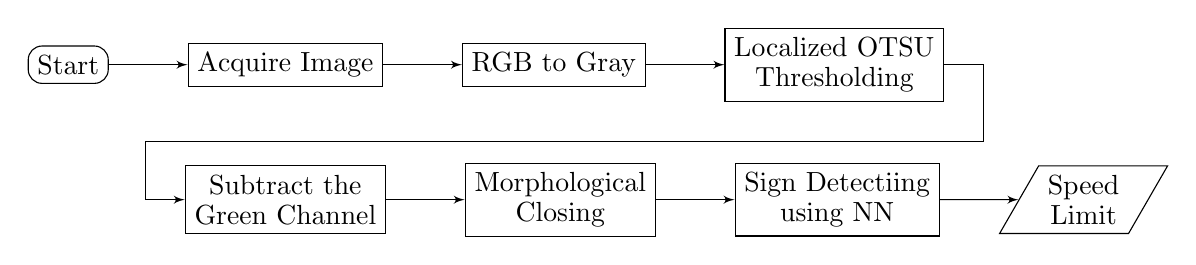
\begin{tikzpicture}[node distance=1cm,>=latex',
block/.style = {draw, shape=rectangle, align=center},
rblock/.style = {draw, shape=rectangle, rounded corners=0.5em},
tblock/.style = {draw, shape=trapezium, trapezium left angle=60, 
	trapezium right angle=120, align=center},
]
\linespread{0.9}
\node [rblock]                      (start)     {Start};
\node [block, right=of start]       (acquire)   {Acquire Image};
\node [block, right=of acquire]     (rgb2gray)  {RGB to Gray};
\node [block, right=of rgb2gray]    (otsu)      {Localized OTSU\\ Thresholding};
\node [block, below=of acquire]     (gchannel)  {Subtract the\\ Green Channel};
\node [block, right=of gchannel]    (closing)   {Morphological\\ Closing};
\node [block, right=of closing]     (detecting) {Sign Detectiing\\ using NN};
\node [tblock, right=of detecting]  (speed)     {Speed\\ Limit};
\draw[->] (start) -- (acquire);
\draw[->] (acquire) -- (rgb2gray);
\draw[->] (rgb2gray) -- (otsu);
\coordinate[below right=5mm and 5mm of otsu]   (a1);
\coordinate[left=5mm of a1 -| gchannel.west]   (a2);
\draw[->] (otsu) -| (a1) -- (a2) |- (gchannel);
\draw[->] (gchannel) -- (closing);
\draw[->] (closing)  -- (detecting);
\draw[->] (detecting) -- (speed);
\end{tikzpicture}



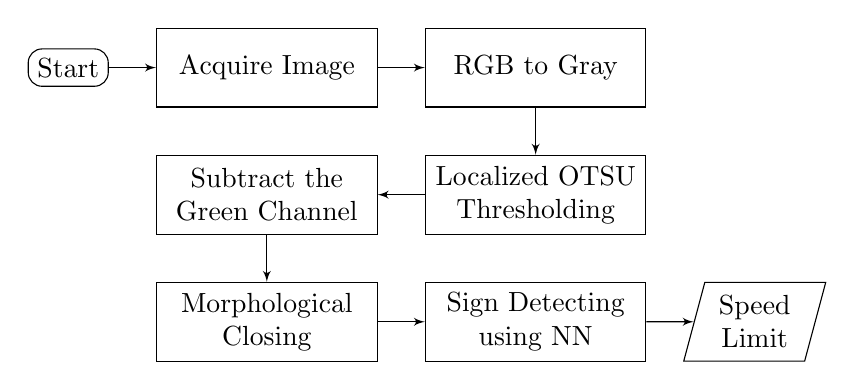
\begin{tikzpicture}[node distance=6mm, >=latex',
block/.style = {draw, rectangle, minimum height=10mm, minimum width=28mm,align=center},
rblock/.style = {draw, rectangle, rounded corners=0.5em},
tblock/.style = {draw, trapezium, minimum height=10mm, 
	trapezium left angle=75, trapezium right angle=105, align=center},
]
\node [rblock]                      (start)     {Start};
\node [block, right=of start]       (acquire)   {Acquire Image};
\node [block, right=of acquire]     (rgb2gray)  {RGB to Gray};
\node [block, below=of rgb2gray]    (otsu)      {Localized OTSU\\ Thresholding};
\node [block, below=of acquire]     (gchannel)  {Subtract the\\ Green Channel};
\node [block, below=of gchannel]    (closing)   {Morphological\\ Closing};
\node [block, right=of closing]     (detecting) {Sign Detecting\\ using NN};
\node [tblock, right=of detecting]  (speed)     {Speed\\ Limit};
%% paths (borowed from Harish Kumar)
\path[draw,->] (start)edge(acquire)    (acquire)edge(rgb2gray)
(rgb2gray)edge(otsu)    (otsu)edge(gchannel)    (gchannel)edge(closing)
(closing)edge(detecting)    (detecting)edge(speed)   ;
\end{tikzpicture}



% ---------------------------------------------------------
\vspace{5ex}

fromhttps://tex.stackexchange.com/questions/306638/simple-block-diagram-tikz

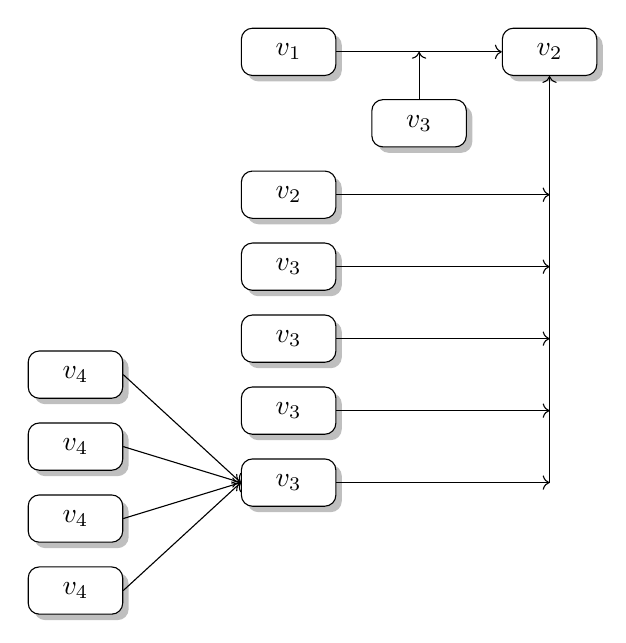
\begin{tikzpicture}[    node distance = 3mm and 21 mm,    start chain = A going below,    every node/.style = {draw, rounded corners, fill=white, minimum width=12mm, minimum height=6mm, drop shadow, on chain=A}    ]   

\node                       {$v_1$};            % A-1
\node[below=12mm of A-1]    {$v_2$};            % A-2
\foreach \i in {1,2,...,4}% since all have the same content
	\node                   {$v_3$};            % A-3 ... A-6
\node[left=of $(A-4)!0.5!(A-5)$]    {$v_4$};    % A-7    % left subcolumn
\foreach \i in {1,2,3}  % since all have the same content
	\node                   {$v_4$};            % A-8 ... A-10                 
\node[right=of A-1]         {$v_2$};            % A-11    % right node
\draw[->] (A-1) -- node[below=6mm] {$v_3$} (A-11);    % arrows top
\draw[->] (A-12) -- (A-1 -| A-12);
\foreach \i in {2,3,...,6}   \draw[->] (A-\i) -- (A-\i -| A-11);    % arrows right
\draw[->] (A-6) -| (A-11);
\foreach \i in {7,8,...,10}   \draw[->] (A-\i.east) -- (A-6.west);    % last arrow left
\end{tikzpicture}



% ---------------------------------------------------------
\vspace{5ex}

from https://texample.net/tikz/examples/consort-flowchart/

\newcommand*{\h}{\hspace{5pt}}% for indentation
\newcommand*{\hh}{\h\h}% double indentation
\begin{center}
	\captionof{figure}{Flowchart of participants' progress through
		the phases of the trial}
	\sffamily 	\footnotesize
	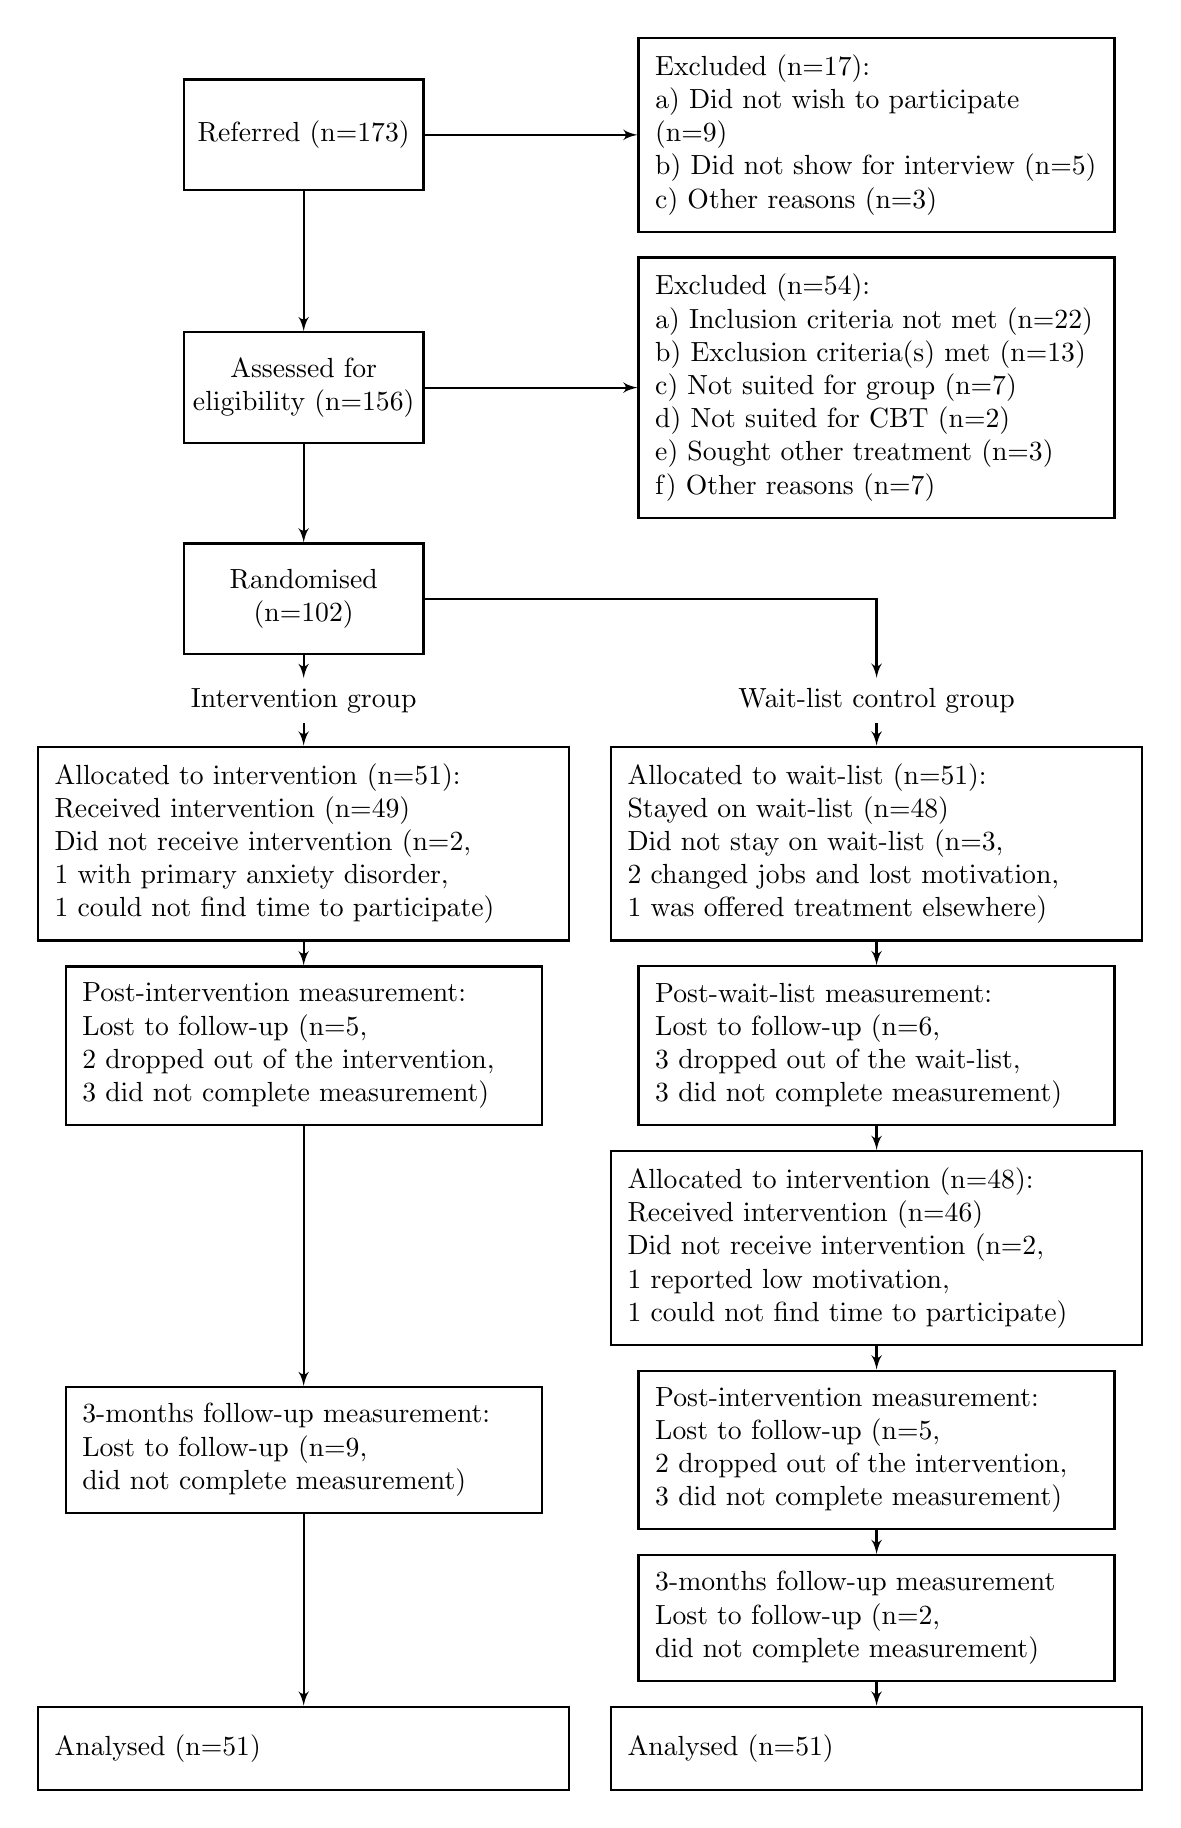
\begin{tikzpicture}[auto,
	%decision/.style={diamond, draw=black, thick, fill=white,
	%text width=8em, text badly centered,
	%inner sep=1pt, font=\sffamily\small},
	block_center/.style ={rectangle, draw=black, thick, fill=white,
		text width=8em, text centered, minimum height=4em},
	block_left/.style ={rectangle, draw=black, thick, fill=white,
		text width=16em, text ragged, minimum height=4em, inner sep=6pt},
	block_noborder/.style ={rectangle, draw=none, thick, fill=none,
		text width=18em, text centered, minimum height=1em},
	block_assign/.style ={rectangle, draw=black, thick, fill=white,
		text width=18em, text ragged, minimum height=3em, inner sep=6pt},
	block_lost/.style ={rectangle, draw=black, thick, fill=white,
		text width=16em, text ragged, minimum height=3em, inner sep=6pt},
	line/.style ={draw, thick, -latex', shorten >=0pt}]
	% outlining the flowchart using the PGF/TikZ matrix funtion
	\matrix [column sep=5mm,row sep=3mm] {
		% enrollment - row 1
		\node [block_center] (referred) {Referred (n=173)};
		& \node [block_left] (excluded1) {Excluded (n=17): \\ a) Did not wish to participate (n=9) \\ b) Did not show for interview (n=5) \\
			c) Other reasons (n=3)}; \\
		% enrollment - row 2
		\node [block_center] (assessment) {Assessed for eligibility (n=156)}; 
		& \node [block_left] (excluded2) {Excluded (n=54): \\ a) Inclusion criteria not met (n=22) \\ b) Exclusion criteria(s) met (n=13) \\
			c) Not suited for group (n=7) \\ d) Not suited for CBT (n=2) \\
			e) Sought other treatment (n=3) \\ f) Other reasons (n=7)}; \\
		% enrollment - row 3
		\node [block_center] (random) {Randomised (n=102)}; 
		& \\
		% follow-up - row 4
		\node [block_noborder] (i) {Intervention group}; 
		& \node [block_noborder] (wlc) {Wait-list control group}; \\
		% follow-up - row 5
		\node [block_assign] (i_T0) {Allocated to intervention (n=51): \\
			\h Received intervention (n=49) \\  \h Did not receive intervention (n=2, \\ 	\hh 1 with primary anxiety disorder, \\ \hh 1 could not find time to participate)}; 
		& \node [block_assign] (wlc_T0) {Allocated to wait-list (n=51): \\
			\h Stayed on wait-list (n=48) \\ \h Did not stay on wait-list (n=3, \\
			\hh 2 changed jobs and lost motivation, \\ \hh 1 was offered treatment elsewhere)}; \\
		% follow-up - row 6
		\node [block_lost] (i_T3) {Post-intervention measurement: \\ \h Lost to follow-up (n=5, \\ \hh 2 dropped out of the intervention, \\ \hh 3 did not complete measurement)}; 
		& \node [block_lost] (wlc_T3) {Post-wait-list measurement: \\ \h Lost to follow-up (n=6, \\ \hh 3 dropped out of the wait-list, \\ \hh 3 did not complete measurement)}; \\
		% follow-up - row 7
		% empty first column for intervention group 
		& \node [block_assign] (wlc_T36) {Allocated to intervention (n=48): \\ 		\h Received intervention (n=46) \\ 	\h Did not receive intervention (n=2, \\
			\hh 1 reported low motivation, \\ \hh 1 could not find time to participate)}; \\
		% follow-up - row 8
		\node [block_lost] (i_T6) {3-months follow-up measurement: \\ \h Lost to follow-up (n=9, \\ \hh did not complete measurement)}; 
		& \node [block_lost] (wlc_T6) {Post-intervention measurement: \\ \h Lost to follow-up (n=5, \\ \hh 2 dropped out of the intervention, \\ \hh 3 did not complete measurement)}; \\
		% follow-up - row 9
		% empty first column for intervention group 
		& \node [block_lost] (wlc_T9) {3-months follow-up measurement \\ \h Lost to follow-up (n=2, \\ \hh did not complete measurement)}; \\
		% analysis - row 10
		\node [block_assign] (i_ana) {Analysed (n=51)}; 
		& \node [block_assign] (wlc_ana) {Analysed (n=51)}; \\
	};% end matrix
	% connecting nodes with paths
	\begin{scope}[every path/.style=line]
	% paths for enrollemnt rows
	\path (referred)   -- (excluded1);
	\path (referred)   -- (assessment);
	\path (assessment) -- (excluded2);
	\path (assessment) -- (random);
	\path (random)     -- (i);
	\path (random)     -| (wlc);
	% paths for i-group follow-up rows
	\path (i)          -- (i_T0);
	\path (i_T0)       -- (i_T3);
	\path (i_T3)       -- (i_T6);
	\path (i_T6)       -- (i_ana);
	% paths for wlc-group follow-up rows
	\path (wlc)        -- (wlc_T0);
	\path (wlc_T0)     -- (wlc_T3);
	\path (wlc_T3)     -- (wlc_T36);
	\path (wlc_T36)    -- (wlc_T6);
	\path (wlc_T6)     -- (wlc_T9);
	\path (wlc_T9)     -- (wlc_ana);
	\end{scope}
	\end{tikzpicture}
\end{center}



% ---------------------------------------------------------

 from https://www.overleaf.com/learn/latex/Pgfplots\_package

%\tikzexternalize
\pgfplotsset{width=10cm,compat=1.9}
\begin{tikzpicture}
\begin{axis}
\addplot[color=red]{exp(x)};
\end{axis}
\end{tikzpicture}

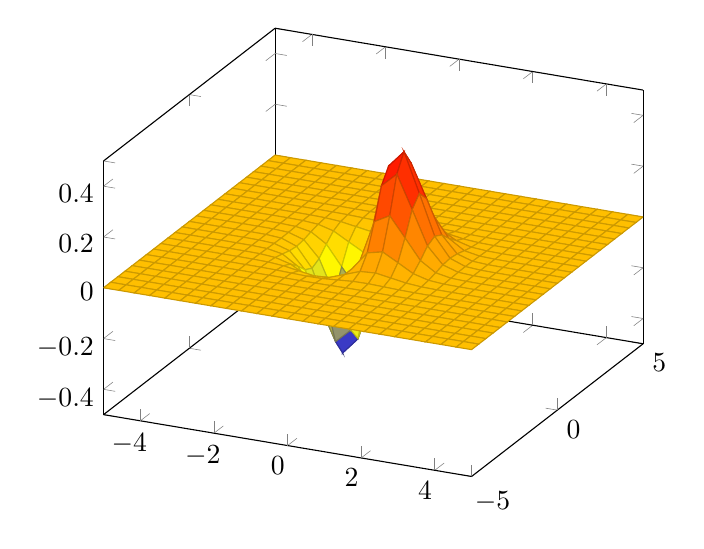
\begin{tikzpicture}
\begin{axis}
\addplot3[surf,]
{exp(-x^2-y^2)*x};
\end{axis}
\end{tikzpicture}


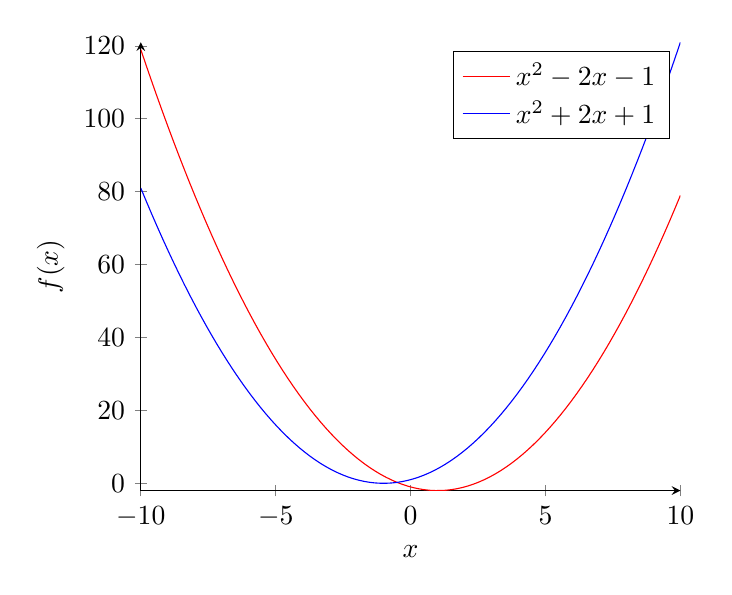
\begin{tikzpicture}
\begin{axis}[axis lines = left,xlabel = \(x\),ylabel = {\(f(x)\)},]
\addplot [domain=-10:10, samples=100, color=red,]
{x^2 - 2*x - 1};
\addlegendentry{\(x^2 - 2x - 1\)}

\addplot [domain=-10:10, samples=100, color=blue,]
{x^2 + 2*x + 1};
\addlegendentry{\(x^2 + 2x + 1\)}
\end{axis}
\end{tikzpicture}


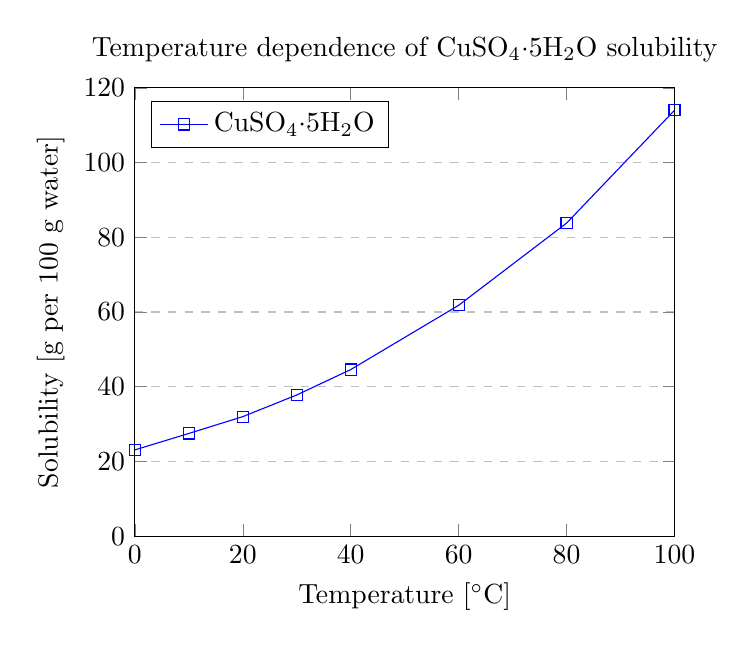
\begin{tikzpicture}
\begin{axis}[title={Temperature dependence of CuSO\(_4\cdot\)5H\(_2\)O solubility},xlabel={Temperature [$^\circ$C]}, ylabel={Solubility [g per 100 g water]}, xmin=0, xmax=100, ymin=0, ymax=120,
xtick={0,20,40,60,80,100}, ytick={0,20,40,60,80,100,120},
legend pos=north west, ymajorgrids=true, grid style=dashed,]
\addplot[color=blue, mark=square,]
coordinates {	(0,23.1)(10,27.5)(20,32)(30,37.8)(40,44.6)(60,61.8)(80,83.8)(100,114)};
\legend{CuSO\(_4\cdot\)5H\(_2\)O}
\end{axis}
\end{tikzpicture}


\begin{tikzpicture}
\begin{axis}[enlargelimits=false,]
	\addplot+[only marks,scatter,mark=halfcircle*,mark size=2.9pt]
	table[meta=ma]{scattered_example.dat};
\end{axis}
\end{tikzpicture}


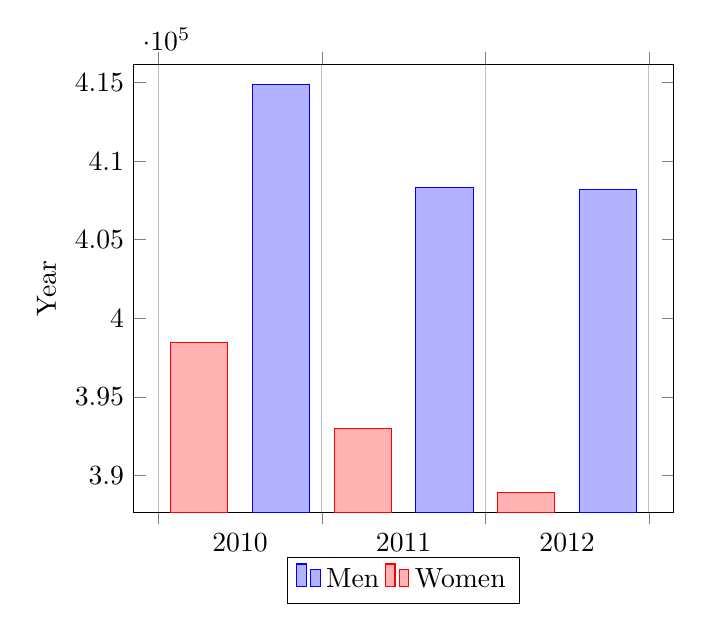
\begin{tikzpicture}
\begin{axis}[x tick label style={/pgf/number format/1000 sep=}, ylabel=Year, enlargelimits=0.05, legend style={at={(0.5,-0.1)}, anchor=north, legend columns=-1}, ybar interval=0.7, ]
\addplot coordinates {(2012,408184) (2011,408348) (2010,414870) (2009,412156)};
\addplot coordinates {(2012,388950) (2011,393007) (2010,398449) (2009,395972)};
\legend{Men,Women}
\end{axis}
\end{tikzpicture}


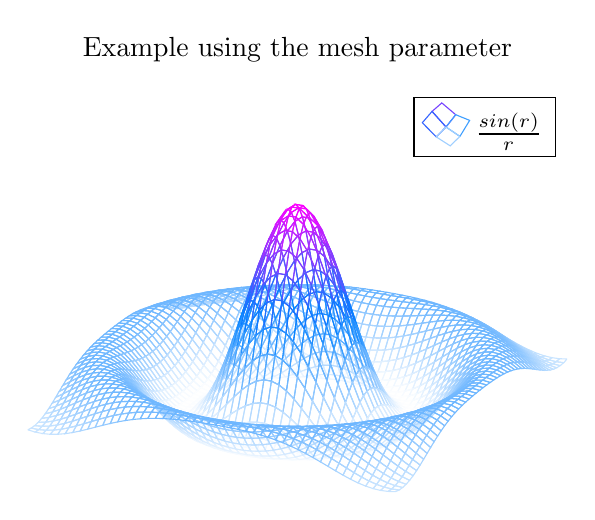
\begin{tikzpicture}
\begin{axis}[title=Example using the mesh parameter,hide axis,colormap/cool,]
\addplot3[mesh, samples=50, domain=-8:8,]
{sin(deg(sqrt(x^2+y^2)))/sqrt(x^2+y^2)};
\addlegendentry{\(\frac{sin(r)}{r}\)}
\end{axis}
\end{tikzpicture}


\begin{tikzpicture}
\begin{axis}[title={Contour plot, view from top}, view={0}{90} ]
\addplot3[contour gnuplot={levels={0.8, 0.4, 0.2, -0.2}} ]
{sin(deg(sqrt(x^2+y^2)))/sqrt(x^2+y^2)};
\end{axis}
\end{tikzpicture}


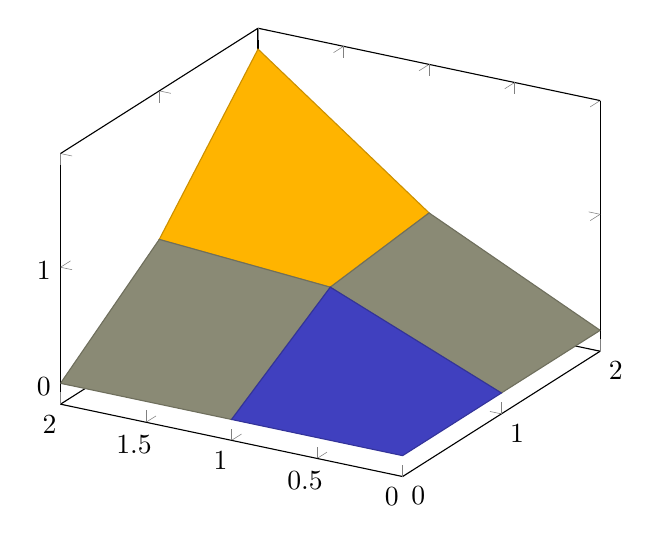
\begin{tikzpicture}
\begin{axis}[view={-60}{30},]
\addplot3[surf,] 
coordinates {(0,0,0) (0,1,0) (0,2,0)
	
	(1,0,0) (1,1,0.6) (1,2,0.7)
	
	(2,0,0) (2,1,0.7)(2,2,1.8)};
\end{axis}
\end{tikzpicture}


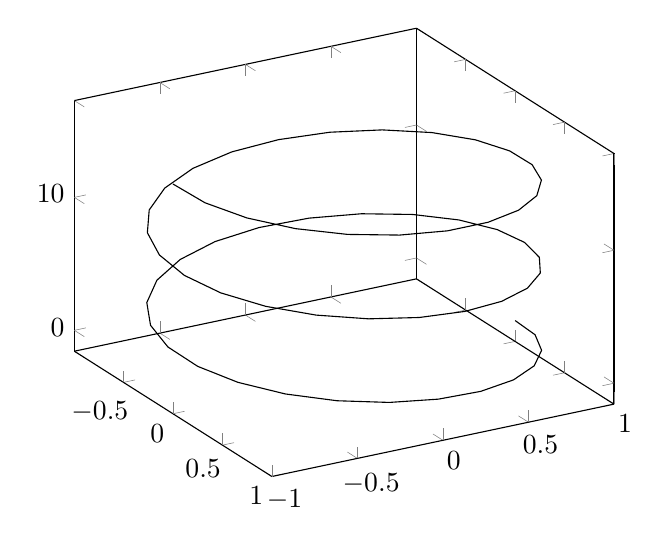
\begin{tikzpicture}
\begin{axis}[view={60}{30},]
\addplot3[domain=0:5*pi,samples = 60,samples y=0,]
({sin(deg(x))},{cos(deg(x))},{x});
\end{axis}
\end{tikzpicture}



% ================================================

from https://stackoverflow.com/questions/36386656/how-to-plot-in-latex-with-gnuplot


\begin{figure}[h]
	\centering
	\begin{gnuplot}[terminal=pdf]
		set terminal pdf enhanced size 14.5cm, 6cm
		set key top left
		set xlabel 'x [1]'
		set ylabel 'y [1]'
		
		f1(x)=sin(x**2)
		
		plot f1(x) title 'y_1 = sin(x^2)'
	\end{gnuplot}
	\caption{Plot}
\end{figure}





\end{document} 